\section{Data Structures}
\subsection*{Disjoint Sets}
A set of sets. Each set has a marked "leader" element.
{\footnotesize Two sets $A$ and $B$ are \textbf{disjoint} if $A\cap B=\emptyset$}

\subsubsection*{Array Representation}
Value in any given index corresponds to its direct parent.
Value will be the same as the index if it is the "root" of a tree set or is just an individual value.

Find: Returns the marked "leader" element of a set.

\subsubsection*{Union Operator}
(prioritize smaller tree height)

Merges two disjoint sets together.
If visualizing as a tree set,
take the tree with the smaller height,
and merge it into the taller tree.

\begin{tikzpicture}[scale=0.4]
    \node (1) at (0,0) {1};
    \node (5) [right=of 1] {$5$}
        child {node (2) {2}
            child {node (8) {8}}
        }
        child {node (4) {4}};
    \node (5a) [right=of 5] {5}
        child {node (2a) {2}
            child {node (8a) {8}}
        }
        child {node (4a) {4}}
        child {node (1a) {1}};
    \node (before) [above=1mm of $(1.north)!0.5!(5.north)$] {Before};
    \node (after) [above=1mm of 5a] {After};
\end{tikzpicture}

\subsubsection*{Path Compression}
(findset on 8)

\begin{tikzpicture}[scale=0.35]
    \node (5) [right=of 1] {$1$}
        child{node (1) {5}
            child {node (2) {2}
                child {node (8) {8}}
            }
            child {node (4) {4}}
        };
    \node (5a) [right=of 5] {1}
        child {node (4a) {2}}
        child {node (1a) {8}}
        child {node (2a) {5}
            child {node (8a) {4}}
        };
    \node (before) [above=1mm of 5] {Before};
    \node (after) [above=1mm of 5a] {After};
\end{tikzpicture}

\arraytable{1}{5}{7}{5}{1}{7}{7}{2}

First, you find the root of this tree which is 1.
Then you go through the path again, starting at 8,
changing the parent of each of the nodes on that path to 1.

\arraytable{1}{5}{7}{5}{1}{7}{7}{1}

Then, you take the 2 that was previously stored in index 8,
and then change the value in that index to 1.

\subsection*{2-4 Trees}

num of children is equal to entries + 1 || 0

\subsubsection*{Insertion}
\resizebox{\linewidth}{!}{%
\begin{tikzpicture}[
    scale=0.1,
    NBox/.style={
        rectangle split,
        rectangle split horizontal,
        draw
    },
    T/.style={
        rectangle split parts=3
    }
    ]
    \node[NBox,T] (root) at (4,0) {\nodepart{two} 3};
    \node[NBox,T] (leftch) [below left=15pt and 5pt of root] {\nodepart{two} 1};
    \node[NBox,T] (leftchrch) [below=15pt and 5pt of leftch.three] {\nodepart{two} 2};
    \node[NBox,T] (leftchlch) [left=15pt and 5pt of leftchrch] {\nodepart{two} 0};
    \node[NBox,rectangle split parts=7] (rightch) [below right=15pt and 5pt of root] {\nodepart{two} 5 \nodepart{four} 7 \nodepart{six} 9};
    \node[NBox,T] (rightchlch) [right=10pt of leftchrch] {\nodepart{two} 4};
    \node[NBox,T] (rightchmch) [right=10pt of rightchlch] {\nodepart{two} 6};
    \node[NBox,T] (rightchrch) [right=10pt of rightchmch] {\nodepart{two} 8};
    \node[NBox,rectangle split parts=7] (rightchchr) [right=10pt of rightchrch] {\nodepart{two} 10 \nodepart{four} 11 \nodepart{six} 12};
    
    \path[->]
    (root.one west) edge [bend right=30] (leftch.two north)
    (leftch.three south) edge (leftchrch.two north)
    (leftch.one south) edge [bend left=15] (leftchlch.two split north)
    (root.three east) edge [bend left=30] (rightch.four north)
    (rightch.one south) edge [bend left=15] (rightchlch.two split north)
    (rightch.three south) edge (rightchmch.two north)
    (rightch.five south) edge [bend right=15] (rightchrch.two split north)
    (rightch.seven east) edge [bend left=15] (rightchchr.three split north);
\end{tikzpicture}
}

{\tiny Insert 13: 4 node. Split it. Push 11 up to parent. Parent is a 4 node, push 7 up.}

\resizebox{\linewidth}{!}{%
\begin{tikzpicture}[
    scale=0.1,
    NBox/.style={
        rectangle split,
        rectangle split horizontal,
        draw
    },
    T/.style={
        rectangle split parts=3
    }
    ]
    \node[NBox,rectangle split parts=5] (root) at (8,0) {\nodepart{two} 3 \nodepart{four} 7};
    \node[NBox,T] (midch) [below=15pt of root] {\nodepart{two} 5};
    \node[NBox,T] (leftch) [left=40pt of midch] {\nodepart{two} 1};
    \node[NBox,T] (leftchrch) [below=15pt and 5pt of leftch.three] {\nodepart{two} 2};
    \node[NBox,T] (leftchlch) [left=15pt and 5pt of leftchrch] {\nodepart{two} 0};
    \node[NBox,rectangle split parts=5] (rightch) [right=40pt of midch] {\nodepart{two} 9 \nodepart{four} 11};
    \node[NBox,T] (rightchlch) [right=10pt of leftchrch] {\nodepart{two} 4};
    \node[NBox,T] (rightchmch) [right=10pt of rightchlch] {\nodepart{two} 6};
    \node[NBox,T] (rightchrch) [right=10pt of rightchmch] {\nodepart{two} 8};
    \node[NBox,T] (rightchchrl) [right=10pt of rightchrch] {\nodepart{two} 10};
    \node[NBox,rectangle split parts=5] (rightchchr) [right=10pt of rightchchrl] {\nodepart{two} 12 \nodepart{four} \color{codegreen}13};
    
    \path[->]
    (root.one west) edge [bend right=30] (leftch.two north)
    (leftch.three south) edge (leftchrch.two north)
    (leftch.one south) edge [bend left=15] (leftchlch.two split north)
    (root.five east) edge [bend left=30] (rightch.two split north)
    (root.three south) edge (midch.two north)
    (midch.one south) edge [bend right=15] (rightchlch.two north)
    (midch.three south) edge (rightchmch.two north)
    (rightch.one south) edge [bend left=15] (rightchrch.two north)
    (rightch.three south) edge [bend right=10] (rightchchrl.two north)
    (rightch.five east) edge [bend left=15] (rightchchr.three split north);
\end{tikzpicture}
}

{\tiny can push up 2nd or 3rd value (3rd is more common)}

\subsubsection*{Deletion}

\begin{enumerate}
    \item Find key to remove and replace w/ next higher key.
    \item If sibling > 1 key, steal an adjacent key, make taht the parent and bring down the current parent.
    \item If no adjacent sibling has greater than one key, steal a key from a parent.
    \item If parent is the root and contains only one key and sibling has only one key, fuse it into a key node and make it the new root.
\end{enumerate}

Delete 20 from the following 2-4 tree.

\resizebox{\linewidth}{!}{%
    \begin{tikzpicture}[
        scale=0.4,
        Node/.style ={
            rectangle split,
            rectangle split horizontal,
            rectangle split parts=#1,
            draw,
        },
        Node/.default=3,
        edge from parent/.style ={draw,-stealth}
    ]
    \node[Node=3] (broot) at (4,0) {
            \nodepart{one} 5
            \nodepart{two} 10
            \nodepart{three} 15
        }
        child {node[Node=1] (b2) {2}
            [parent anchor=one south]
        }
        child {node[Node=1] (b6) {6}
            [parent anchor=two south]
        }
        child {node[Node=1] (b13) {13}
            [parent anchor=two south]
        }
        child {node[Node=1] (b20) {20}
            [parent anchor=three south]
        };

    \node[Node=2] (aroot) [right=of broot] {
            \nodepart{one} 5
            \nodepart{two} 10
        }
        child {node[Node=1] (a2) {2}
            [parent anchor=one south]
        }
        child {node[Node=1] (a6) {6}
            [parent anchor=two south]
        }
        child {node[Node=2] (a13) [right=0.8em of a6] {
                \nodepart{one} 13
                \nodepart{two} 15
            }
            [parent anchor=two south]
        };

    \node (before) [above=1mm of broot] {Before};
    \node (after) [above=1mm of aroot] {After};

    \end{tikzpicture}
}
\subsection*{Binary Tree Relationships}
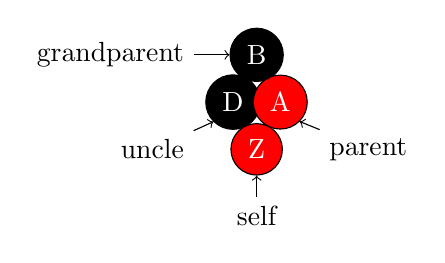
\begin{tikzpicture}[
    scale=0.4,
    blk/.style ={
        circle,
        white,
        fill=black,
        draw=black
    },
    rd/.style ={
        circle,
        white,
        fill=red,
        draw=black
    }
    ]
    \node[blk] (grandparent) at (0,0) {B}
        child{node[blk] (uncle) {D}}
        child{node[rd] (parent) {A}
              child{node[rd] (self) {Z}}
              child[missing]};

    \path[->] +(-2,0) node[left] {grandparent} edge (grandparent.west);
    \path[->] +(-2,-3) node[left] {uncle} edge (uncle.south west);
    \path[->] +(2,-3) node[right] {parent} edge (parent.south east);
    \path[->] +(0,-4.5) node[below] {self} edge (self.south);
\end{tikzpicture}

\subsection*{Red-Black Trees}
\begin{enumerate}
    \item A node is either {\color{red}red} or black.
    \item The root and leaves (NIL) are black.
    \item If a node is {\color{red}red}, then its children are black.
    \item All paths from a node to its NIL descendants contain the same number of black nodes.
    \item The longest path (root to farthest NIL) is no more than twice the length of the shortest path (root to nearest NIL).
        \scriptsize{
        \begin{itemize}
            \item Shortest path: all black nodes
            \item Longest path: alternating {\color{red}red} and black
        \end{itemize}}
\end{enumerate}

\subsubsection*{Insertion}
Strategy:
\begin{enumerate}
    \item Insert Z and color it {\color{red}red}
    \item Recolor and rotate nodes to fix violation
\end{enumerate}
{\bfseries Z is illegal scenarios}
\begin{enumerate}%
    \item[0.] Z = root $\to$ color black
    \item[1.] Z.uncle = {\color{red}red} $\to$ recolor
    \item[2.] {\scriptsize Z.uncle = {\bfseries black}(triangle) $\to$ rotate Z.parent}\\
        \resizebox{!}{5em}{% Black triangle diagram
        \begin{tikzpicture}[
            scale=0.4,
            blk/.style ={
                circle,
                white,
                fill=black,
                draw=black
            },
            rd/.style ={
                circle,
                white,
                fill=red,
                draw=black
            }
            ]
            \node[blk] (grandparent) at (0,0) {B}
                child{node[blk] (uncle) {C}}
                child{node[rd] (parent) {A}
                    child{node[rd] (self) {Z}}
                    child[missing]};

            \path[->,blue] ($(parent)+(0,0.8)$) edge [in=120,out=45] ($(parent)+(0.75,0.5)$);

            \node () [above right=1mm of grandparent] {Z right child, parent left child \& vice-versa};

            \node[blk] (agrandparent) [right=5em of grandparent] {B}
                child{node[blk] (auncle) {C}}
                child{node[rd] (aparent) {Z}
                    child[missing]
                    child{node[rd] (aself) {A}}};

            \path[->] (parent.east) ++(0.25,0) edge ($(auncle.west)+(-0.25,0)$);

            %% Mirrored

            \node[blk] (mgrandparent) [right=5em of agrandparent] {B}
                child{node[rd] (muncle) {C}
                    child[missing]
                    child{node[rd] (mself) {Z}}
                }
                child{node[blk] (mparent) {A}};

            \path[->,blue] ($(muncle)+(0,0.8)$) edge [in=45,out=120] ($(muncle)+(-0.75,0.5)$);

            \node[blk] (magrandparent) [right=5em of mgrandparent] {B}
                child{node[rd] (mauncle) {Z}
                    child{node[rd] (maself) {C}}
                    child[missing]
                }
                child{node[blk] (maparent) {A}};

            \path[->] (mparent.east) ++(0.25,0) edge ($(mauncle.west)+(-0.25,0)$);

            %% Anti-confusion mirror line
            \draw[draw] let \p1 = ($(aself)!0.5!(muncle)$),
                \p2 = (maself) in ($(\x1,0)$) -- +(0,\y2);
            %% Above line is overly complicated for what it is

        \end{tikzpicture}
        }
    \item[3.] {\scriptsize Z.uncle = {\bfseries black}(line) $\to$ rotate Z.grandparent \& recolor}\\
        \resizebox{!}{5em}{% Black line diagram
        \begin{tikzpicture}[
            scale=0.4,
            blk/.style ={
                circle,
                white,
                fill=black,
                draw=black
            },
            rd/.style ={
                circle,
                white,
                fill=red,
                draw=black
            }
            ]
            \node[blk] (grandparent) at (0,0) {B}
                child{node[blk] (uncle) {C}}
                child{node[rd] (parent) {A}
                    child{node[blk] (sib) {D}}
                    child{node[rd] (self) {Z}}
                };
            \path[->,blue] ($(grandparent)+(0,0.8)$) edge [in=45,out=120] ($(grandparent)+(-0.75,0.5)$);
            \path[->,blue] ($(parent.north east)+(0.1,0)$) edge +(120:1);
            \node () [above right=1mm of grandparent] {Z and parent are same side children};
            \node[blk] (agrandparent) [right=5em of grandparent] {A}
                child{node[rd] (aparent) {B}
                    child{node[blk] (asib) {C}}
                    child{node[blk] (aself) {D}}
                }
                child{node[rd] (auncle) {Z}};
            \path[->] (parent.east) ++(0.25,0) edge ($(aparent.west)+(-0.25,0)$);

            %% Mirrored

            \node[blk] (mgrandparent) [right=5em of agrandparent] {B}
                child{node[rd] (muncle) {C}
                    child{node[rd] (mself) {Z}}
                    child{node[blk] (msib) {D}}
                }
                child{node[blk] (mparent) {A}};
            \path[->,blue] ($(mgrandparent)+(0,0.8)$) edge [in=120,out=45] ($(mgrandparent)+(0.75,0.5)$);
            \path[->,blue] ($(muncle.north west)+(-0.1,0)$) edge +(60:1);
            \node[blk] (magrandparent) [right=5em of mgrandparent] {C}
                child{node[rd] (maparent) {Z}}
                child{node[rd] (mauncle) {B}
                    child{node[blk] (maself) {D}}
                    child{node[blk] (masib) {A}}
                };
            \path[->] (mparent.east) ++(0.25,0) edge ($(maparent.west)+(-0.25,0)$);

            %% Anti-confusion mirror line
            \draw[draw] let \p1 = ($(auncle)!0.5!(mself)$),
                \p2 = (maself) in ($(\x1,0)$) -- +(0,\y2);
            %% Above line is overly complicated for what it is

        \end{tikzpicture}%
        }
\end{enumerate}

\subsubsection*{Deletion}

DB node has\ldots
\begin{enumerate}%
    \item {\bfseries\color{black}black sibling with at least one red child.}
        This fixes the problem structurally. No extra work is required
        after this case completes. This corresponds to a transfer operation in a 2-4 Tree.
    \item {\bfseries\color{black}black sibling with two black children.}
        This uses recoloring and no structural change. It may solve the problem, but
        may ALSO propagate the DB node to the parent of the current DB node. This corresponds
        to a fusion and drop operation in a 2-4 Tree.
    \item {\bfseries\color{black}red sibling.}
        A structural change here puts you in case 1 or case 2.
        At this point, a single application of either case is sufficient.
        This corresponds to a fusion where you have enough values in the parent node to drop
        one into the fused child.
\end{enumerate}

\subsubsection*{Convert from a 2-4 Tree}
Strategy:
\begin{enumerate}%
    \item Each {\bfseries\color{black}2-Node} should be colored {\bfseries\color{black}black}.
    \item Each {\bfseries\color{black}3-Node} should be converted into {\bfseries\color{black}2} nodes, with its parent node being {\bfseries\color{black}black} and child being {\bfseries\color{red}red}.
    \item Each {\bfseries\color{black}4-Node} should be converted into {\bfseries\color{black}3} nodes, with its parent node being {\bfseries\color{black}black} and {\bfseries\color{black}2} children being {\bfseries\color{red}red}.
\end{enumerate}

Example:

\resizebox{\linewidth}{!}{%
\begin{tikzpicture}[
        scale=0.4,
        level/.style={sibling distance=20em/#1},
    ]
    \node (1020) [right=of 1] {10,20}
        child {node (357) {3,5,7}
                child {node (1b) {1}}
                child {node (4b) {4}}
                child {node (6b) {6}}
                child {node[xshift=-2em] (8b) {8}} % manually shifting cause tis fucked
        }
        child{node (1) {15}
            child {node (2) {2}
                child {node (8) {12,13}}
                child {node (17) {17}}
            }
            child {node (4) {4}}
        }
        child {node (2530) {25,30}
            child {node (21b) {21}}
            child {node (27b) {27}}
            child {node (32b) {32}}
        };
    \node (before) [above=1mm of 1020] {Before};
\end{tikzpicture}
}

\resizebox{\linewidth}{!}{%
\begin{tikzpicture}[
        scale=0.4, 
        level/.style={sibling distance=20em/#1},
    ]
    \node (10a) [right=of 1] {10}
        child {node (5a) {5}
                child {node (3a) {{\bfseries\color{red}3}}
                    child {node (1a) {1}}
                    child {node (4a) {4}}
                }
                child {node (7a) {{\bfseries\color{red}7}}
                    child {node (6a) {8}}
                    child {node (8a) {8}}
                }
                child {node (6b) {6}}
                child {node[xshift=-2em] (8b) {8}} % manually shifting cause tis fucked
        }
        child{node (20a) {{\bfseries\color{red}20}}
            child {node (15a) {15}
                child {node (12a) {12}
                    child {node (13a) {{\bfseries\color{red}13}}}
                }
                child {node (17a) {17}}
            }
            child {node (30a) {30}
                child {node (25a) {{\bfseries\color{red}25}}
                    child {node (21a) {21}}
                    child {node (27a) {27}}
                }
                child {node (32a) {32}}
            }
        };
    \node (before) [above=1mm of 10a] {After};
\end{tikzpicture}
}

\subsection*{Skip Lists}
Stacks of linked lists.
\subsubsection*{Insertion}
Insert at bottom level. 50\% chance it's added up, again \& again. Stop if it is only one at top level.
\subsubsection*{Deletion}
Delete value and update all pointers.
%TODO: More Info
